\PassOptionsToPackage{table}{xcolor}
%\documentclass{beamer}
\documentclass[handout]{beamer}

\setbeamertemplate{bibliography item}{\insertbiblabel}

\usepackage[utf8]{inputenc}
\usepackage{algorithm, algorithmic}
\usepackage{caption}
\usepackage{mathtools}
\usepackage{mathrsfs}
\usepackage{tabularx}
\usepackage{color, colortbl}
\usepackage{array, booktabs, ragged2e}
\usepackage{makecell}
\usepackage{tikz}
\usepackage{textpos}

\definecolor{RowColorOdd}{rgb}{0.914,0.914,0.953}
\definecolor{RowColorEven}{rgb}{1,1,1}

\definecolor{lightgray}{rgb}{0.83, 0.83, 0.83}

\renewcommand\theadfont{\bfseries}

\usepackage[backend=biber]{biblatex}
\addbibresource{References.bib}

\DeclareMathOperator{\balance}{balance}
\DeclareMathOperator{\argmin}{argmin}
\DeclareMathOperator{\aggregate}{AGGREGATE}
\DeclareMathOperator{\combine}{COMBINE}
\DeclareMathOperator{\readout}{READOUT}
\DeclareMathOperator{\MAX}{MAX}
\DeclareMathOperator{\MEAN}{MEAN}
\DeclareMathOperator{\relu}{ReLU}
\DeclareMathOperator{\concat}{CONCAT}
\DeclareMathOperator{\mlp}{MLP}
\DeclareMathOperator{\hash}{HASH}
\DeclareMathOperator{\gin}{GIN}

\renewcommand*{\bibfont}{\tiny}

\usetheme{Madrid}
\usecolortheme{default}

%------------------------------------------------------------
%This block of code defines the information to appear in the
%Title page
\title[How Powerful are Graph Neural Networks?]
{How Powerful are Graph Neural Networks?}

\subtitle{(EE531 Final Project - Graph)}

\author[Junghyun Lee]
{K.~Xu\inst{1} \and W.~Hu\inst{2} \and J.~Leskovec\inst{2} \and S.~Jegelka\inst{1}}

\institute[KAIST]
{
	\inst{1}%
	MIT
	
	\inst{2}%
	Stanford University
}

\date[ICLR 2019]
{Appeared at ICLR 2019}


%End of title page configuration block
%------------------------------------------------------------



%------------------------------------------------------------
%The next block of commands puts the table of contents at the 
%beginning of each section and highlights the current section:

\AtBeginSection[]
{
  \begin{frame}
    \frametitle{Outline}
    \tableofcontents[currentsection]
  \end{frame}
}

\AtBeginSubsection[]
{
  \begin{frame}
    \frametitle{Outline}
    \tableofcontents[currentsection, currentsubsection]
  \end{frame}
}
%------------------------------------------------------------


\begin{document}

%The next statement creates the title page.
\frame{\titlepage}


%---------------------------------------------------------
%This block of code is for the table of contents after
%the title page
\begin{frame}
\frametitle{Table of Contents}
\tableofcontents
\end{frame}
%---------------------------------------------------------

\section{Introduction}

%---------------------------------------------------------
\begin{frame}
\frametitle{Introduction}
\setbeamerfont{footnote}{size=\tiny}

\begin{itemize}
    \item Since GNN(Graph Neural Network) has come out, it has revolutionized the field of representation learning, especially with graph datas. \pause
    \item But why GNNs work? Why are they so powerful? \pause
    \item Most interestingly, {\it how powerful are they?}
\end{itemize}
\end{frame}

%---------------------------------------------------------

\section{Previous / Related Works}

%---------------------------------------------------------
\begin{frame}
\frametitle{Previous / Related Works}
\setbeamerfont{footnote}{size=\tiny}

\begin{itemize}
    \item There hasn't been much work regarding this topic.\pause
    \item Scarselli et al.\footfullcite{Scarselli2009b} showed that the (probably) earliest GNN model\footfullcite{Scarselli2009a} can approximate measurable functions in probability.\pause
    \item Lei et al.\footfullcite{Lei2017} showed that their architecture lies in the RKHS of graph kernels, {\it but do not study explicitly which graph it can distinguish.}\pause
    \item Above works focus on a specific architecture and {\bf do not easily generalize to other architectures}.\pause
    \item This paper presents a \alert{general framework} for analyzing/characterizing the expressive power of a \alert{broad class of GNNs}!
\end{itemize}
\end{frame}

%---------------------------------------------------------

\section{Preliminaries}

%---------------------------------------------------------

\subsection{GNNs}

%---------------------------------------------------------
\begin{frame}
\frametitle{GNN}

\begin{itemize}
	\item Let $G = (V, E)$ be a graph, or data with graph structure. \pause
	
	\item Each $v \in V$ has a {\it node feature vector}, $X_v$ \pause
	
	\item There are two tasks of interest where GNN is commonly used: \pause
\end{itemize}

\begin{block}{Node Classification Problem}
Each $v \in V$ has an associated label $y_v$.

{\bf Goal:} Learn a representation vector $h_v$ of $v$ such that $y_v = f(h_v)$ i.e. such that $v$'s label can be predicted. 
\end{block} \pause

\begin{block}{Graph Classification Problem}
A set of graphs $\{G_1, \dots, G_N\} \subset \mathcal{G}$ is given, along with their labels $\{y_1, \dots, y_N\} \subset \mathcal{Y}$.

{\bf Goal:} Learn a representation vector $h_G$ of $G$ such that $y_G = f(h_G)$ i.e. such that $G$'s label can be predicted. 
\end{block}

\end{frame}

%---------------------------------------------------------
\begin{frame}
\frametitle{GNN}

\begin{itemize}
	\item Modern GNNs follow a \alert{neighborhood aggregation strategy} (message passing strategy) \pause
	
	\item Iteratively update the representation of a nodes by aggregating representations of its neighbors! \pause
	
	\item Let $h_v^{(k)}$ is the feature vector of node $v$ at the $k$-th iteration/layer, and let us initialize it as $h_v^{(0)} = X_v$. \pause
	
	\item $k$-th layer of a GNN is
	
	$$a_v^{(k)} = \aggregate^{(k)} \left( \left\{ h_u^{(k - 1)} : u \in \mathcal{N}_G(v) \right\} \right)$$
	$$h_v^{(k)} = \combine^{(k)} \left( h_v^{(k - 1)}, a_v^{(k)} \right)$$
\end{itemize}

\end{frame}

%---------------------------------------------------------
\begin{frame}
\frametitle{GNN}
\setbeamerfont{footnote}{size=\tiny}

\begin{itemize}
	\item Different choices of $\aggregate^{(k)}$ and $\combine^{(k)}$ have led to different GNN variants/architectures. \pause
	
	\item GraphSAGE\footfullcite{Hamilton2017}:
	$$a_v^{(k)} = \MAX \left( \left\{ \relu \left( W h_u^{(k - 1)} \right) : u \in \mathcal{N}_G(v) \right\} \right)$$
	$$h_v^{(k)} = W \left[ h_v^{(k - 1)}, a_v^{(k)} \right]$$ \pause
	
	\item Graph Convolutional Networks, or GCN\footfullcite{Kipf2017}:
	$$h_v^{(k)} = \relu \left( W \MEAN \left\{ h_u^{(k - 1)} : u \in \mathcal{N}_G(v) \cup \{v\} \right\} \right)$$
\end{itemize}

\end{frame}

%---------------------------------------------------------
\begin{frame}
\frametitle{GNN}
\setbeamerfont{footnote}{size=\tiny}

\begin{itemize}
	\item In case of node classification, the final node representation $h_v^{(K)}$ is used for prediction. \pause
	
	\item In case of graph classification, the final node representations are aggregated by $\readout$ function to obtain the entire graph's representation:
	$$h_G = \readout \left( \left\{ h_v^{(K)} : v \in V \right\} \right)$$ \pause
	
	\item $\readout$ can be a simple permutation invariant function, or something more sophisticated\footfullcite{Ying2018}\footfullcite{Zhang2018}
\end{itemize}

\end{frame}

%---------------------------------------------------------

\subsection{WL test}

%---------------------------------------------------------
\begin{frame}
\frametitle{Graph Isomorphism Problem}

\begin{itemize}
	\item Consider the following problem: \pause
	
\begin{block}{\textsc{Graph Isomorphism (GI)}}
{\bf Input}:  Two finite graphs $G_1$ and $G_2$

{\bf Question}: $G_1 \cong G_2$?

\end{block} \pause

	\item Appears in: discrete mathematics, mathematical logic, theory of computation, machine learning, computer vision...etc. \pause
	
	\item This seemingly harmless problem has harassed researchers for decades!
\end{itemize}

\end{frame}

%---------------------------------------------------------
\begin{frame}
\frametitle{Graph Isomorphism Problem}
\setbeamerfont{footnote}{size=\tiny}

Here are some facts related to \textsc{GI}:

\begin{itemize}
	\item Not known to be of class NP-complete nor tractable!
	
	(Researchers have actually defined a new complexity class {\bf GI}) \pause
	
	\item It is currently known that \textsc{GI} can be solved in quasipolynomial time {\it i.e.} in $O \left( 2^{O \left( \left( \log n \right)^c \right)} \right) (c > 0)$ time\footfullcite{Babai2016}: \pause
	
\begin{block}{Theorem (Babai, 2015)}
The Graph Isomorphism problem ... can be solved in quasipolynomial time.
	\end{block}
(Confirmed by Harald Andr\'es Helfgott, probably correct)	
	 \pause

	\item But it is not practical! \pause
	
	\item Some practical algorithms: McKay (1981), Schmidt \& Druffel (1976), Ullman (1976)...etc.
\end{itemize}

\end{frame}

%---------------------------------------------------------
\begin{frame}
\frametitle{Weisfeiler-Lehman test}
\setbeamerfont{footnote}{size=\tiny}

\begin{itemize}
	\item Weisfeiler-Lehman test of graph isomorphism\footfullcite{Weisfeiler1968}, or simply WL test, is a combinatorial algorithm for \textsc{GI}. \pause
	
	\item WL test is proved to be successful (and computationally efficient) in isomorphism testing for a broad class of graphs\footfullcite{Babai1979} \pause
	
	\item There are some cases (ex. regular graphs) when the WL test fails\footfullcite{Cai1992}
\end{itemize}

\end{frame}

%---------------------------------------------------------
\begin{frame}
\frametitle{Weisfeiler-Lehman test}

\begin{itemize}
	\item Why are we interested in this WL test? \pause
	
	\item 1-dimensional form of the WL test ("na\"ive vertex refinement") is {\it based on neighbor aggregations}, analogous to the GNNs! \pause
	
	\item Overview of the algorithm:
	\begin{itemize}
		\item Aggregate the labels of nodes and their neighborhoods
		\item Hashes the aggregated label into {\it unique} new labels
		\item If at some iteration the labels of the nodes between the two graphs differ, then the two graphs are non-isomorphic.
	\end{itemize}
	
\end{itemize}

\end{frame}

%---------------------------------------------------------
\begin{frame}
\frametitle{1-dim WL test}

Let $(G, l)$ be a labeled graph i.e. a graph $G$ with an endowed node coloring $l : V(G) \rightarrow \Sigma$.
($\Sigma$: arbitrary codomain) \pause

\begin{itemize}
	\item At $t$-th iteration ($t \geq 0$), the 1-WL computes a node coloring $c_l^{(t)} : V(G) \rightarrow \Sigma$, which depends on the previous node coloring:
	$$c_l^{(0)} = l, \ c_l^{(t)}(v) = \hash \left( \left( c_l^{(t - 1)}(v), \{\{ c_l^{(t - 1)}(u) | u \in \mathscr{N}(v) \}\} \right) \right)$$	
($\hash$ bijectively maps the above pair to a unique value in $\Sigma$ that hasn't been used in previous iterations)	
	\pause
	
	\item Run above algorithm in parallel for the two input graphs. \pause
	
	\item If at some iteration, the two graphs have a different number of nodes colored $\sigma \in \Sigma$, conclude that the graphs are not isomorphic. \pause
	
	(This why this 1-dim version is commonly called the {\it color refinement algorithm})
\end{itemize}

\end{frame}

%---------------------------------------------------------
\begin{frame}
\frametitle{WL subtree kernel}
\setbeamerfont{footnote}{size=\tiny}

\begin{itemize}
	\item \alert{Graph kernel}: kernel function that defines {\it inner product on graphs} \footfullcite{Vishwanathan2010}
	
(Function measuring the similarity of a pair of two given graphs) \pause

	\item Some examples: {\it random walk} (G\"artner {\it et al.}, 2003; Borgwardt {\it et al.}, 2005), {\it marginalized} (Kashima {\it et al.}, 2003, 2004; Mah\'e {\it et al.}, 2004) \pause
	
	\item \alert{Weisfeiler-Lehman subtree kernel}\footfullcite{Shervashidze2011}: counts common {\it original and compressed labels} (resulting from 1-dim WL test) in two graphs.
\end{itemize}

\end{frame}

%---------------------------------------------------------
\begin{frame}
\frametitle{WL subtree kernel}

\begin{figure}[hbt]
	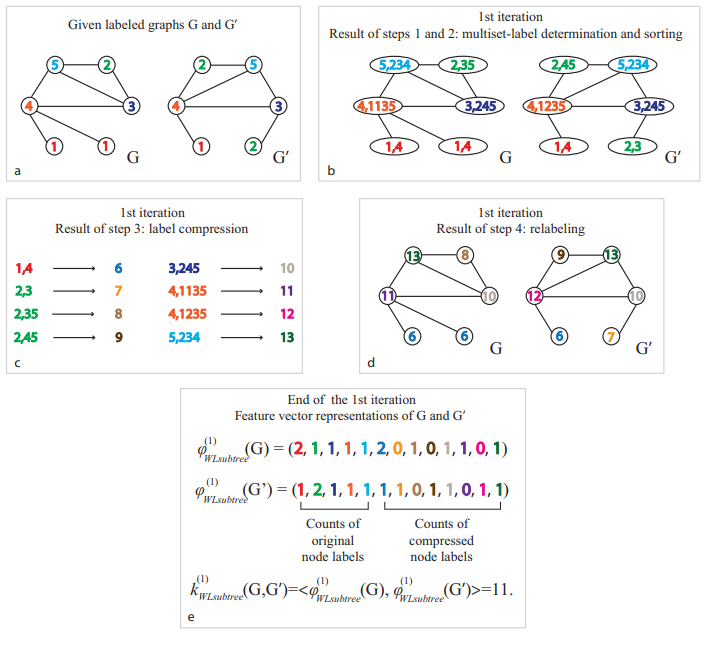
\includegraphics[height=8cm]{fig1.png}
\end{figure}

\end{frame}

%---------------------------------------------------------
\begin{frame}
\frametitle{WL subtree kernel}

\begin{itemize}
	\item Is it related to GNN? \pause Yes! \pause
	
	\item The kernel uses the {\it counts of node labels} at different iterations of the WL test as the {\it feature vector} of a graph. \pause
	
	\item Intuitively, a node’s label at the $k$-th iteration of the 1-dim WL test represents a subtree structure of height k rooted at the node.

	\begin{figure}[hbt]
		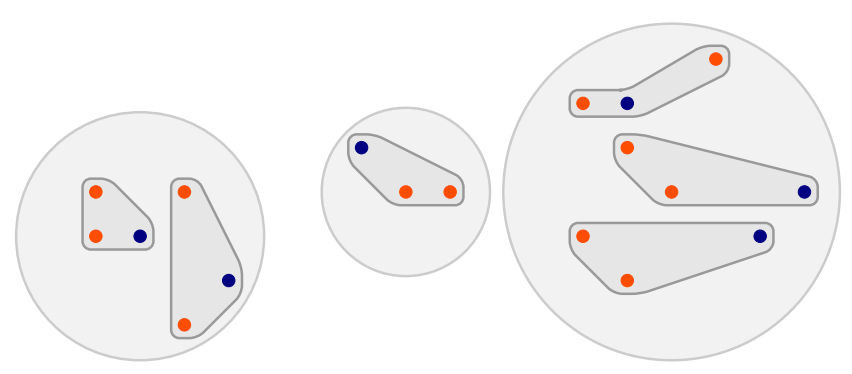
\includegraphics[height=2.5cm]{fig2.png}
	\end{figure}

	\item Thus, the graph features considered by the WL subtree kernel are essentially counts of different rooted subtrees in the graph!

\end{itemize}

\end{frame}

%---------------------------------------------------------
\begin{frame}
\frametitle{k-dim WL test}
\setbeamerfont{footnote}{size=\tiny}

\begin{itemize}
	\item k-dim WL test is a generalization of the 1-dim WL test; it colors tuples from $V(G)^k$ instead of nodes. \pause
	
	\item Why would we want to do that? \pause
	
	\item  By increasing $k$, the algorithm gets more powerful in terms of distinguishing non-isomorphic graphs!   \pause

	\item It was shown that for each $k \geq 2$, there are non-isomorphic graphs which can be distinguished by the $(k + 1)$-dim WL test, but not by the $k$-dim WL test\footfullcite{Cai1992} \pause
	
	\item In this work, we only focus on 1-dim WL test.
\end{itemize}

\end{frame}

%---------------------------------------------------------
\subsection{(Overview of) Theoretical Framework}

%---------------------------------------------------------
\begin{frame}
\frametitle{(Overview of) Theoretical Framework}

\begin{figure}[hbt]
	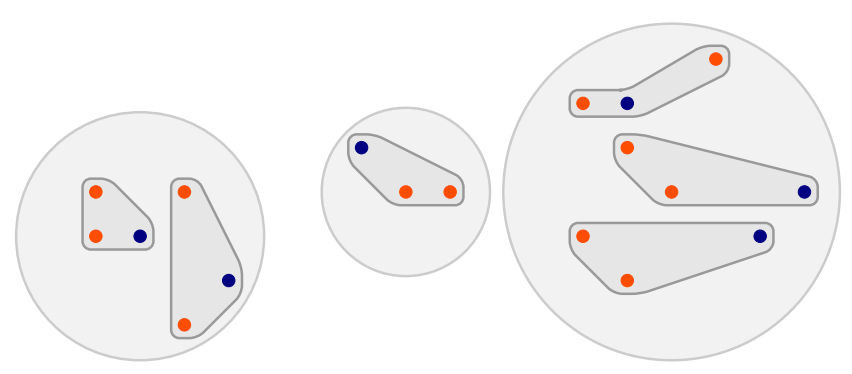
\includegraphics[height=3cm]{fig2.png}
\end{figure}

\begin{itemize}
    \item GNN: recursive update of each node's feature vector {\it i.e.} its rooted subtree structure! \pause
    
    \item ($1$-dim) WL test: also results in rooted subtree structure! \pause
    
    \item Assign each feature vector a unique label from a countable universe. \pause
    
    \item Then, feature vectors of a set of neighboring nodes form a \alert{multiset}.
\end{itemize}
\end{frame}

%---------------------------------------------------------
\begin{frame}
\frametitle{(Overview of) Theoretical Framework}

\begin{figure}[hbt]
	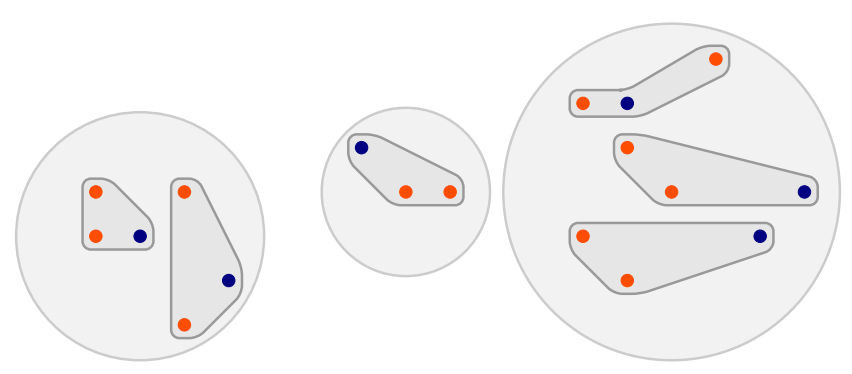
\includegraphics[height=3cm]{fig2.png}
\end{figure}

\begin{itemize}
    \item Representational power of a GNN: when a GNN maps two nodes to the same location (in the embedding space)? \pause
    
    \item Maximally powerful GNN: its aggregation scheme must be \alert{injective}! \pause
    
    \item Closely related to \textsc{Graph Isomorphism}. \pause
    
    \item GNN's aggregation scheme: {\it class of functions over multisets that their neural networks can represent}
\end{itemize}
\end{frame}

%---------------------------------------------------------

\section{Representational capacity of GNNs}

%---------------------------------------------------------
\begin{frame}
\frametitle{Representational capacity of GNNs}

\begin{itemize}
	\item Recall: maximally powerful GNN has injective aggregation scheme. \pause
	
	\item Two (non)isomorphic graphs are mapped to the (different)same representation(s). \pause
	
	\item Characterized by \textsc{Graph Isomorphism}! \pause
	
	\begin{block}{Lemma 2}
Let $G_1$ and $G_2$ be any two non-isomorphic graphs.

If a graph neural network $\mathcal{A} : \mathcal{G} \rightarrow \mathbb{R}^d$ maps $G_1$ and $G_2$ to different embeddings, the Weisfeiler-Lehman graph isomorphism test also decides $G_1$ and $G_2$ are not isomorphic.
	\end{block} \pause

	\item It says that \alert{any aggregation-based GNN is {\it at most} as powerful as the WL test} in distinguishing different graphs.
\end{itemize}

\end{frame}

%---------------------------------------------------------
\begin{frame}
\frametitle{Representational capacity of GNNs}

\begin{itemize}
	\item Is that "bound" tight? \pause
	
	\item In other words, does there exist GNN that is, in principle, as powerful as the WL test in distinguishing different graphs? \pause

\begin{block}{Theorem 3}
Let $\mathcal{A} : \mathcal{G} \rightarrow \mathbb{R}^d$ be a GNN.

With a sufficient number of GNN layers, $\mathcal{A}$ maps any $G_1$ and $G_2$ that the Weisfeiler-Lehman test of isomorphism decides as non-isomorphic, to different embeddings if the following conditions hold:

\begin{itemize}
\item $\mathcal{A}$ aggregates and updates node features iteratively with
$$h_v^{(k)} = \phi \left( h_v^{(k - 1)}, f \left( \left\{ h_u^{(k - 1)} : u \in \mathcal{N}_G(v) \right\} \right) \right)$$
where the functions $f$, which operates on multisets, and $\phi$ are {\it injective}.
\item $\mathcal{A}$'s graph-level readout, which operates on the multiset of node features $\left\{ h_v^{(k)} \right\}$, is {\it injective}.
\end{itemize}
\end{block}
\end{itemize}

\end{frame}

%---------------------------------------------------------
\begin{frame}
\frametitle{Representational capacity of GNNs}

\begin{itemize}
	\item Node feature vectors in the WL test are essentially one-hot encodings, and thus cannot capture similarity between subtrees! \pause
	
	\item GNN (satisfying the criteria in Theorem 3) generalizes the WL test by {\it learning to embed} the subtrees to low-dimensional space. \pause
	
	\item GNNs can not only discriminate different structures, but can also \alert{learn to map similar graph structures to similar embeddings and {\it capture dependencies between graph structures}}. \pause
	
	\item Especially useful when co-occurence of subtrees is sparse across different graphs, or there are noisy edges and node features.\footfullcite{Yanardag2015}
\end{itemize}

\end{frame}

%---------------------------------------------------------

\section{Graph Isomorphism Network (GIN)}

%---------------------------------------------------------
\begin{frame}
\frametitle{Graph Isomorphism Network (GIN)}
\setbeamerfont{footnote}{size=\tiny}

\begin{itemize}
	\item Well we've proved (or more accurately, seen) that GNNs under certain conditions is maximally powerful. \pause
	
	\item Let us develop a simple architecture, GIN! \pause
	
	\item Idea: \alert{deep multisets}\footfullcite{Zaheer2017} {\it i.e.} parametrizing universal multiset functions with neural networks.

\end{itemize}


\end{frame}

%---------------------------------------------------------
\begin{frame}
\frametitle{Graph Isomorphism Network (GIN)}

\begin{itemize}
\begin{block}{Lemma 5}
Assume $\mathcal{X}$ is countable.
There exists a function $f : \mathcal{X} \rightarrow \mathbb{R}^n$ so that $h(X) = \sum_{x \in X} f(x)$ is unique for each multiset $X \subset \mathcal{X}$ of bounded size.

Moreover, any multiset function $g$ can be decomposed as $g(X) = \phi \left( \sum_{x \in X} f(x) \right)$ for some function $\phi$.
\end{block} \pause

	\item Observe that certain popular injective set functions, such as the mean aggregator, are {\it not} injective multiset functions! \pause
	
	\item This lemma tells us that sum aggregators can represent injective, in fact, {\it universal} functions over multisets. \pause
	
	\item Thus, we can conceive aggregation schemes that can \alert{represent universal functions over a node and the multiset of its neighbors}, satisfying the {\it injectiveness condition} (a) in Theorem 3!

\end{itemize}


\end{frame}

%---------------------------------------------------------
\begin{frame}
\frametitle{Graph Isomorphism Network (GIN)}
\setbeamerfont{footnote}{size=\tiny}

\begin{itemize}

	\item Here is a simple and concrete formulation of the previous discussion:
	
\begin{block}{Corollary 6}
Assume $\mathcal{X}$ is countable.
There exists a function $f : \mathcal{X} \rightarrow \mathbb{R}^n$ so that for infinitely many choices of $\epsilon$, including all irrational numbers, $h(c, X) = (1 + \epsilon) f(c) + \sum_{x \in X} f(x)$ is unique for each pair $(c, X)$, where $c \in \mathcal{X}$ and $X \subset \mathcal{X}$ is a multiset of bounded size.

Moreover, any function $g$ over such pairs can be decomposed as $g(c, X) = \varphi \left( (1 + \epsilon) f(c) + \sum_{x \in X} f(x) \right)$ for some function $\varphi$.
\end{block} \pause

	\item We can use MLPs to model and learn $f$ and $\varphi$, thanks to the Universal Approximation Theorem\footfullcite{Hornik1989}\footfullcite{Hornik1991}.
\end{itemize}

\end{frame}

%---------------------------------------------------------
\begin{frame}
\frametitle{How powerful is MLP?}

\begin{block}{Universal Approximation Theorem (Hornik, 1991)}
Define
$$\mathscr{N}_k^{(n)} (\psi) = \left\{ h : \mathbb{R}^k \rightarrow \mathbb{R} \middle| h(x) = \sum_{j = 1}^n \beta_j \psi(a_j' x - \theta_j) \right\}$$
as the set of all functions implemented by such a network with $n$ hidden units, where $\psi$ is the common activation function of the hidden units.

{\it If $\psi$ is continuous, bounded and nonconstant, then $\mathscr{N}_k^{(n)} (\psi)$ is dense in $\mathscr{C}(X)$ for all compact subsets $X$ of $\mathbb{R}^k$.}
\end{block} \pause

\begin{itemize}
	\item Every continuous function can be approximated arbitrarily closely by a multi-layer perceptron with just one hidden layer. \pause
	
	\item The choice of the activation function doesn't matter; it's the multilayer feedforward architecture that gives neural networks the potential of being universal approximators.
\end{itemize}

\end{frame}

%---------------------------------------------------------
\begin{frame}
\frametitle{Graph Isomorphism Network (GIN)}
\setbeamerfont{footnote}{size=\tiny}

\begin{itemize}
	\item In practice, $f^{(k + 1)} \circ \varphi^{(k)}$ is modeled with one MLP.\pause
	
	\item We may make $\epsilon$ as a learnable parameter, or a fixed scalar.\pause
	
	\item Then, $\gin$ updates node representations as:
	$$h_v^{(k)} = \mlp^{(k)} \left( \left(1 + \epsilon^{(k)} \right) h_v^{(k - 1)} + \sum_{u \in \mathscr{N}(v)} h_u^{(k - 1)} \right)$$
\end{itemize}

\end{frame}


%---------------------------------------------------------
\begin{frame}
\frametitle{Graph Isomorphism Network (GIN)}
\setbeamerfont{footnote}{size=\tiny}

\begin{itemize}
	\item Node embeddings, learned by the GIN, can be directly used for node classification and link prediction. \pause
	
	\item For graph classification tasks, we need a $\readout$ function. \pause
	
	\item We want to consider all structural information, considering that features from earlier iterations may sometimes generalize better. \pause
	
	\item Use information from {\it all} depths/iterations of the model\footfullcite{Xu2018}!
	
	$$h_G = \concat \left( \readout \left( \left\{ h_v^{k} | v \in V(G) \right\} \right) \middle| k = 0, 1, \dots, K \right)$$ \pause
	
	\item Note that if $\gin$ replaces $\readout$ with summing all node features from the same iteration, it provably generalizes the WL test and the WL subtree kernel.
\end{itemize}

\end{frame}

%---------------------------------------------------------

\section{Less powerful, but still interesting GNNs}

%---------------------------------------------------------
\begin{frame}
\frametitle{Overview}

\begin{itemize}
	\item Now we consider GNNs that do not satisfy the conditions as described in Theorem 3 and/or GNNs with different choice of $\aggregate$ (Max-pooling, Mean) \pause
	
	\item What if 1-layer perceptron is used instead of $\mlp$s? \pause
	
	\item What if the sum $h(X) = \sum_{x \in X} f(x)$ is replaced by mean/max pooling?
	
\end{itemize}
\end{frame}

%---------------------------------------------------------

\subsection{1-Layer Perceptrons}

%---------------------------------------------------------
\begin{frame}
\frametitle{MLP?}
\setbeamerfont{footnote}{size=\tiny}

\begin{itemize}
	\item The function $f$ in Lemma 5 helps map distinct multisets to unique embeddings. \pause
	
	\item $f$ can be parametrized by MLPs, as shown by the Universal Approximation Theorem\footfullcite{Hornik1991}
	
\end{itemize}

\end{frame}

%---------------------------------------------------------


%---------------------------------------------------------
\begin{frame}
\frametitle{Without MLP?}

\begin{itemize}
	\item Many modern GNNs, however, use a {\it 1-layer perceptron} $\sigma \circ W$: a linear mapping followed by a non-linear activation function. \pause
	
	\item Is 1-layer perceptron enough for graph learning? \pause

\begin{block}{Lemma 7}
There exist finite multisets $X_1 \not= X_2$ so that for any linear mapping $W$, $\sum_{x \in X_1} \relu(Wx) = \sum_{x \in X_2} \relu(Wx)$
\end{block} \pause

	\item Unlike models using MLPs, 1-layer perceptron (even with the bias term) is \alert{not a universal approximator of multiset functions}.
	
\end{itemize}

\end{frame}

%---------------------------------------------------------

\subsection{GCN}

%---------------------------------------------------------
\begin{frame}
\frametitle{GCN}
\setbeamerfont{footnote}{size=\tiny}

\begin{itemize}
	\item As described previously, Graph Convolutional Network\footfullcite{Kipf2017} takes the form:
	$$h_v^{(k)} = \relu \left( W \MEAN \left\{ h_u^{(k - 1)} : u \in \mathcal{N}_G(v) \cup \{v\} \right\} \right)$$ \pause
	
	\item GCN utilizes mean aggregator. \pause
	
	\item How can we characterize the structures that GCN can or cannot capture?
\end{itemize}

\end{frame}

%---------------------------------------------------------
\begin{frame}
\frametitle{Mean aggregator}

\begin{itemize}
	\item Consider two multisets $X_1 = (S, m)$ and $X_2 = (S, k m)$ \pause
	
	\item Observation: Any mean aggregator maps $X_1$ and $X_2$ to the {\it same} embeddings! \pause
	
	\item Mean aggregator captures the \alert{distribution of elements in a multiset}. \pause

\begin{block}{Corollary 8}
Assume $\mathcal{X}$ is countable.
There exists a function $f : \mathcal{X} \rightarrow \mathbb{R}^n$ so that $h(X) = \frac{1}{|X|}\sum_{x \in X} f(x)$, $h(X_1) = h(X_2)$ {\it if only if} multisets $X_1$ and $X_2$ hav e the same distribution.
That is, assuming $|X_2| \geq |X_1|$, we have $X_1 = (S, m)$ and $X_2 = (S, k m)$ for some $k \in \mathbb{N}$.

\end{block} \pause

	\item This is as powerful as the sum aggregator if the node features are diverse and rarely repeat, and thus {\it effective for node classification}.

\end{itemize}
\end{frame}

%---------------------------------------------------------


\subsection{GraphSAGE}

%---------------------------------------------------------
\begin{frame}
\frametitle{GraphSAGE}
\setbeamerfont{footnote}{size=\tiny}

\begin{itemize}
	\item As described previously, GraphSAGE\footfullcite{Hamilton2017} takes the form:
	$$a_v^{(k)} = \MAX \left( \left\{ \relu \left( W h_u^{(k - 1)} \right) : u \in \mathcal{N}_G(v) \right\} \right)$$
	$$h_v^{(k)} = W \left[ h_v^{(k - 1)}, a_v^{(k)} \right]$$ \pause
	
	\item GraphSAGE utilizes max-pooling aggregator. \pause
	
	\item How can we characterize the structures that GraphSAGE can or cannot capture?
\end{itemize}

\end{frame}

%---------------------------------------------------------
\begin{frame}
\frametitle{Max-pooling aggregator}

\begin{itemize}
	\item Unlike previous aggregators, max-pooling can't capture exact structure nor the distribution! \pause
	
	\item But it can capture the \alert{underlying set of muliset} {\it i.e.} $S$ in $X = (S, m)$ \pause

\begin{block}{Corollary 9}
Assume $\mathcal{X}$ is countable.
There exists a function $f : \mathcal{X} \rightarrow \mathbb{R}^\infty$ so that $h(X) = \max_{x \in X} f(x)$, $h(X_1) = h(X_2)$ {\it if only if} multisets $X_1$ and $X_2$ have the same underlying set.

\end{block}

\end{itemize}
\end{frame}

%---------------------------------------------------------
\begin{frame}
\frametitle{Summary}

\begin{itemize}
	\item Let us rank the three aggregators by their representational power: \pause

\begin{figure}[hbt]
  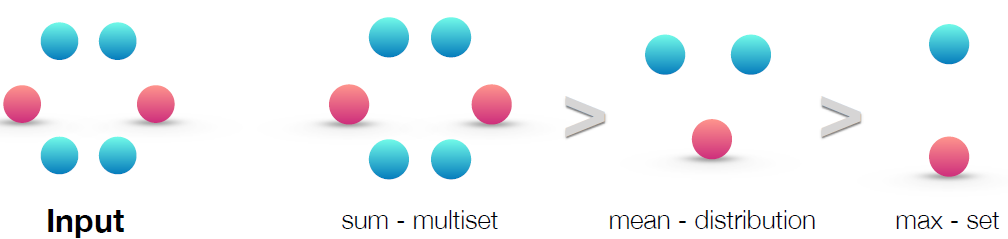
\includegraphics[height=2cm]{fig3.png}
\end{figure} \pause

\begin{figure}[hbt]
  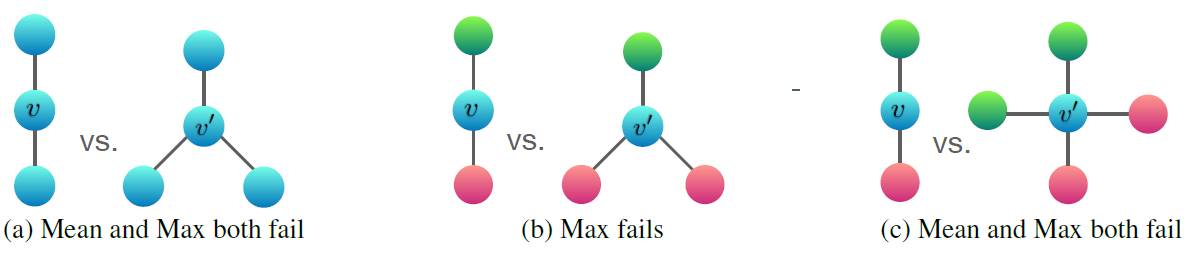
\includegraphics[height=2cm]{fig4.png}
\end{figure}

	\item Sum over multiset aggregator (as in GIN) completely captures the exact structure of graph. \pause
		
	\item Mean aggregator (as in GCN) captures the statistical and distributional information of the graph. \pause
	
	\item Max-pooling aggregator (as in GraphSAGE) captures the representative elements of the graph, or its skeleton
\end{itemize}


\end{frame}

%---------------------------------------------------------

\section{Experiments}

%---------------------------------------------------------
\begin{frame}
\frametitle{Experiments}

The goal of the experiment is to compare the training and test performance of $\gin$ and less powerful GNN variants. \pause

\begin{itemize}
	\item Training set performance: compare different GNN models based on their {\it representational power}

	\item Test set performance: quantifies {\it generalization ability}
\end{itemize}

\end{frame}

%---------------------------------------------------------


%---------------------------------------------------------
\begin{frame}
\frametitle{Experiment Design}

\begin{itemize}
	\item 9 graph classification benchmarks were used\footfullcite{Yanardag2015}:
	\begin{itemize}
		\item 4 bioinformatics datasets ({\it MUTAG, PTC, NCI1, PROTEINS})
		\item 5 social network datasets ({\it COLLAB, IMDB-BINARY, IMDB-MULTI, REDDIT-BINARY, REDDIT-MULTI5K})
	\end{itemize} \pause
	
	\item Several models were used:
	\begin{itemize}
		\item $\gin-\epsilon$: $\gin$ that {\it learns} $\epsilon$ by gradient descent
		\item $\gin-0$: $\gin$ that fixes $\epsilon$ to $0$.
		\item Architectures that replace the sum in the $\gin-0$ aggregation with mean or max-pooling, or replace MLPs with 1-layer perceptrons
		\item GCN
		\item GraphSAGE
	\end{itemize} \pause
	
	\item The baselines used were:
	\begin{itemize}
		\item WL subtree kernel with $C$-SVM used as a classifier
		\item Deep learning architectures i.e. DCNN, PATCHY-SAN, DGCNN
		\item AWL
	\end{itemize}
\end{itemize}

\end{frame}

%---------------------------------------------------------


%---------------------------------------------------------
\begin{frame}
\frametitle{Results}

\begin{figure}[hbt]
  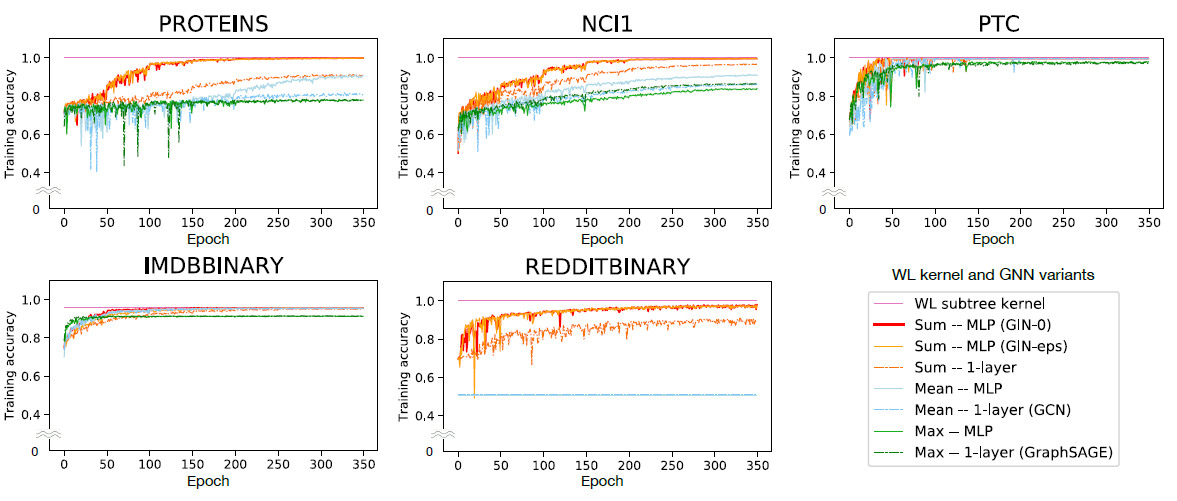
\includegraphics[height=5cm]{fig5.png}
\end{figure}

\end{frame}

%---------------------------------------------------------
\begin{frame}
\frametitle{Results}

\begin{figure}[hbt]
  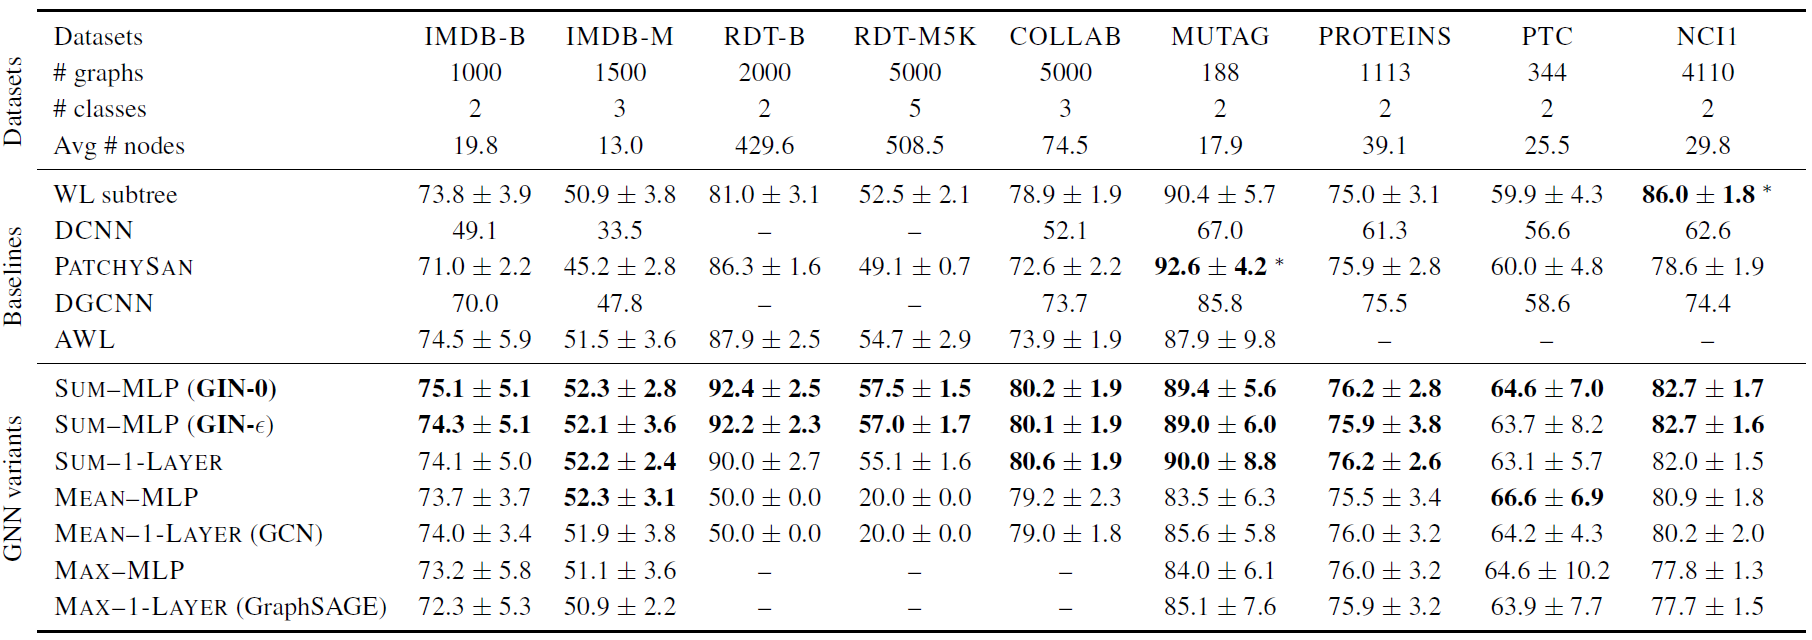
\includegraphics[height=4cm]{fig6.png}
\end{figure}

\end{frame}

%---------------------------------------------------------

\section{Summary / Future Research}

%---------------------------------------------------------
\begin{frame}
\frametitle{Summary}

In summary, \pause

\begin{itemize}
	\item Theoretical foundations for reasoning about the expressive power of GNNS \pause

	\item Tight bounds on the representational capacity of popular GNN variants. (cf. WL test) \pause

	\item Designed a provably maximally powerful GNN under the neighborhood aggregation framework ({\it Graph Isomorphism Network})
	
\end{itemize}

\end{frame}

%---------------------------------------------------------
\begin{frame}
\frametitle{Future research}

\begin{itemize}
	\item Different aggregators? \pause
	\item Go beyond neighborhood aggregation \pause
	\item Understand/improve the generalization properties of GNNs \pause
	\item What if the node features are continuous (uncountable)? \pause
	\item Better understanding of the optimization landscape
\end{itemize}

\end{frame}

%---------------------------------------------------------

\section{Summary of GNNs}

%---------------------------------------------------------
\begin{frame}
\frametitle{Summary of GNNs}
\setbeamerfont{footnote}{size=\tiny}

Here is a summary of "major" GNNs\footfullcite{Wu2019}: (next page)

\end{frame}

%---------------------------------------------------------
\begin{frame}
\frametitle{Summary of GNNs}

(1: RecGNN, 2: Spectral-based ConvGNN, 3: Spatial-based ConvGNN)

\resizebox{\columnwidth}{!}{%

\begin{tabular}{|llll|}
\toprule
\thead{Method} & \thead{Category} & \thead{Time \\ Complexity} & \thead{Features} \\

\hline
\rowcolor{lightgray}
GNN\cite{Scarselli2009b} & $1$ & $O(m)$ & Information diffusion mechanism, updates nodes' states until a stable equilibrium is reached.\\

Spectral CNN\cite{Bruna2014} & $2$ & $O(n^3)$ & Treats the filters as a set of learnable parameters.\\

\rowcolor{lightgray}
ChebNet\cite{Defferrard2016} & $2$ & $O(m)$ & Approximates the filger by Chebyshev polynomials of the diagonal matrix of eigenvalues.\\

GCN\cite{Kipf2017} & $2$ & $O(m)$ & First-order approximation of ChebNet\\

\rowcolor{lightgray}
AGCN\cite{Li2018} & $2$ & $O(n^2)$ & Learns hidden structural relations by using the residual graph adjacency matrix through learnable metric.\\

DualGCN\cite{Zhuang2018} & $2$ & $O(m)$ & Introduces dual graph convolutional architecture with two graph convolutional layers in parallel.\\

\rowcolor{lightgray}
NN4G\cite{Micheli2009} & $3$ & $O(m)$ & Performs graph convolutions by summing up a node's neighborhood information directly.\\

DCNN\cite{Atwood2016} & $3$ & $O(n^2)$ & Treats graph convolutions as a diffusion process\\

\rowcolor{lightgray}
MPNN\cite{Gilmer2017} & $3$ & $O(m)$ & Treats graph convolutions as a message passing process.\\

GraphSAGE\cite{Hamilton2017} & $3$ & - & Sampling of fixed number of neighbors for each node.\\

\rowcolor{lightgray}
\alert{GIN}\cite{Xu2019} & $3$ & $O(m)$ & This paper!\\

\bottomrule
\end{tabular}
}

\end{frame}

%---------------------------------------------------------

\section{References}

%---------------------------------------------------------

\begin{frame}[allowframebreaks]
\frametitle{References}
\nocite{*}
\printbibliography
\end{frame}

%---------------------------------------------------------

\begin{frame}{}
  \centering \Large
  \emph{Thank you for your attention! Any questions?}
\end{frame}

%---------------------------------------------------------

\end{document}